% Article de vulgarisation en quatre planches A3 (chacune une double page de magazine).
% Compiler : cd docs/vulgarisation && tectonic -X compile article-a3.tex
\documentclass[10pt]{article}
\usepackage{fontspec}
\setmainfont{Charter}
\newfontfamily\titre{Avenir Next}[UprightFont=* Bold, BoldFont=* Heavy]
\newfontfamily\sans{Avenir Next}[UprightFont=* Regular, BoldFont=* Demi Bold, ItalicFont=* Italic]
\newfontfamily\sanscond{Avenir Next Condensed}[UprightFont=* Demi Bold]
\usepackage{polyglossia}\setmainlanguage{french}
\usepackage[a3paper,landscape,margin=14mm,top=13mm,bottom=12mm]{geometry}
\usepackage{multicol,graphicx,xcolor,tcolorbox,microtype,amssymb,needspace,tikz}
\usetikzlibrary{calc}
\usepackage[hidelinks]{hyperref}
\setlength{\columnsep}{5mm}
\setlength{\parindent}{1em}
\setlength{\parskip}{0pt}
\definecolor{bleu}{HTML}{38539D}
\definecolor{orange}{HTML}{E0612B}
\definecolor{encre}{HTML}{2B2A27}
\definecolor{gris}{HTML}{6F6B63}
\definecolor{papier}{HTML}{F4EFE6}
\pagestyle{empty}
\newlength{\demi}\setlength{\demi}{\dimexpr(\textwidth-18mm)/2\relax}
% Une planche = deux pages côte à côte, séparées par la pliure.
\newcommand{\planche}[2]{\noindent\begin{minipage}[t][\dimexpr\textheight-8pt][t]{\demi}\vspace{0pt}#1\end{minipage}\hspace{18mm}\begin{minipage}[t][\dimexpr\textheight-8pt][t]{\demi}\vspace{0pt}#2\end{minipage}\newpage}
\newcommand{\surtitre}[1]{{\sanscond\color{orange}\fontsize{11}{13}\selectfont\MakeUppercase{#1}}}
\newcommand{\rubrique}[1]{{\sanscond\color{orange}\fontsize{10}{12}\selectfont\MakeUppercase{#1}}\par\vspace{1mm}}
\newcommand{\grandtitre}[1]{{\titre\color{encre}\fontsize{30}{33}\selectfont #1}\par\vspace{3mm}}
\newcommand{\chapo}[1]{{\sans\fontsize{12.5}{17}\selectfont\color{encre}#1}\par\vspace{4mm}}
\newcommand{\inter}[1]{\par\needspace{5\baselineskip}\medskip{\sans\bfseries\color{bleu}\fontsize{11}{13}\selectfont #1}\par\nobreak\smallskip\noindent\ignorespaces}
\newcommand{\legende}[1]{{\sans\fontsize{8.2}{10.4}\selectfont\color{gris}#1}}
\newcommand{\exergue}[1]{\par\medskip{\titre\color{orange}\fontsize{16}{19}\selectfont «\,#1\,»}\par\smallskip}
\newcommand{\lettrine}[1]{{\titre\fontsize{30}{30}\selectfont\color{bleu}#1}}
\newtcolorbox{encadre}[1]{colback=papier,colframe=papier,arc=0pt,boxrule=0pt,left=3mm,right=3mm,top=2.5mm,bottom=2.5mm,fontupper=\sans\fontsize{8.8}{11.4}\selectfont,title={\sans\bfseries\fontsize{10.5}{12}\selectfont\color{orange}#1},coltitle=orange,colbacktitle=papier,toptitle=1mm}
\newcommand{\folio}[1]{\par\vfill\noindent\rule{\linewidth}{0.3pt}\par\vspace{1mm}\noindent{\sans\fontsize{7.5}{9}\selectfont\color{gris}Les cartons secrets de Grothendieck\hfill #1}}
\newcommand{\foliog}[1]{\par\vfill\noindent\rule{\linewidth}{0.3pt}\par\vspace{1mm}\noindent{\sans\fontsize{7.5}{9}\selectfont\color{gris}#1\hfill Les cartons secrets de Grothendieck}}
% Pseudo-droites dessinées comme des droites dans un disque.
\newcommand{\ligne}[3][bleu]{\draw[#1,line width=1pt,shorten <=-6cm,shorten >=-6cm] (#2) -- (#3);}
\newcommand{\disque}{\draw[gris!70,dashed] (0,0) circle (1.6); \clip (0,0) circle (1.6);}
\makeatletter\renewcommand\normalsize{\@setfontsize\normalsize{11.4}{15.2}}\makeatother

\begin{document}\normalsize

% =================================================================== planche 1 (pages 1-2)
\planche{%
\surtitre{Mathématiques · Archives}\par\vspace{4mm}
{\raggedright\hyphenpenalty=10000\titre\color{encre}\fontsize{58}{60}\selectfont Les cartons secrets de~Grothendieck\par}\vspace{6mm}
{\raggedright\sans\fontsize{14}{19}\selectfont\color{encre}En 1970, l'un des mathématiciens les plus influents du XX\textsuperscript{e} siècle quitte la recherche officielle. Il n'a pourtant jamais cessé d'écrire. Seize mille pages de ses brouillons dorment à Montpellier, vingt-deux mille feuillets à la Bibliothèque nationale. Une machine les a lus. Voici ce qu'elle y a trouvé, et ce qu'elle a manqué.\par}\vspace{3mm}
{\sans\fontsize{9}{11}\selectfont\color{gris}Par Michel Hua}\par\vspace{6mm}
\noindent\rule{\linewidth}{0.6pt}\par\vspace{4mm}
\begin{multicols}{2}
\noindent\lettrine{D}ans les années 1960, Alexandre Grothendieck a refait de fond en comble la géométrie algébrique, cette branche des mathématiques qui étudie les figures définies par des équations. Ses traités, les EGA et les SGA, comptent ensemble environ huit mille pages imprimées ; on y apprend encore aujourd'hui. Médaille Fields en 1966, il quitte en 1970 l'Institut des hautes études scientifiques, rompt avec le milieu, s'installe dans le Sud de la France et finit sa vie retiré dans un village des Pyrénées, où il meurt en 2014.

On a longtemps cru qu'après 1970 il avait plus ou moins arrêté les mathématiques. Ses papiers racontent autre chose. En 1990 et 1995, il confie ses manuscrits mathématiques à Jean Malgoire, un ancien élève. Déposés à l'université de Montpellier en 2010, donnés en 2012, ils sont aujourd'hui en libre accès : 178 dossiers, 16\,074 pages numérisées. Le reste, ses écrits des années 1987 à 1999, est entré à la BnF : 43 boîtes, 22\,495 feuillets.

\inter{Des brouillons sans date}
Le problème, c'est que presque personne ne les a lus. Une vingtaine de dossiers ont été édités à la main par des mathématiciens, dont les célèbres \emph{Dérivateurs} et le premier volume d'\emph{À la poursuite des champs}. Les autres sont des notes de travail à l'encre et au crayon, reprises, raturées, annotées, dans une notation qui lui est propre.

Et elles ne sont presque jamais datées. Sur 164 dossiers transcrits, Grothendieck n'a daté ses feuillets de sa main que dans vingt et un, presque tous des années 1981 à 1986. Les dates de l'inventaire sont pour la plupart déduites par les archivistes, d'après un verso, une lettre, un dossier voisin, ou la date imprimée sur du papier de récupération.

\end{multicols}
\folio{1}}{%
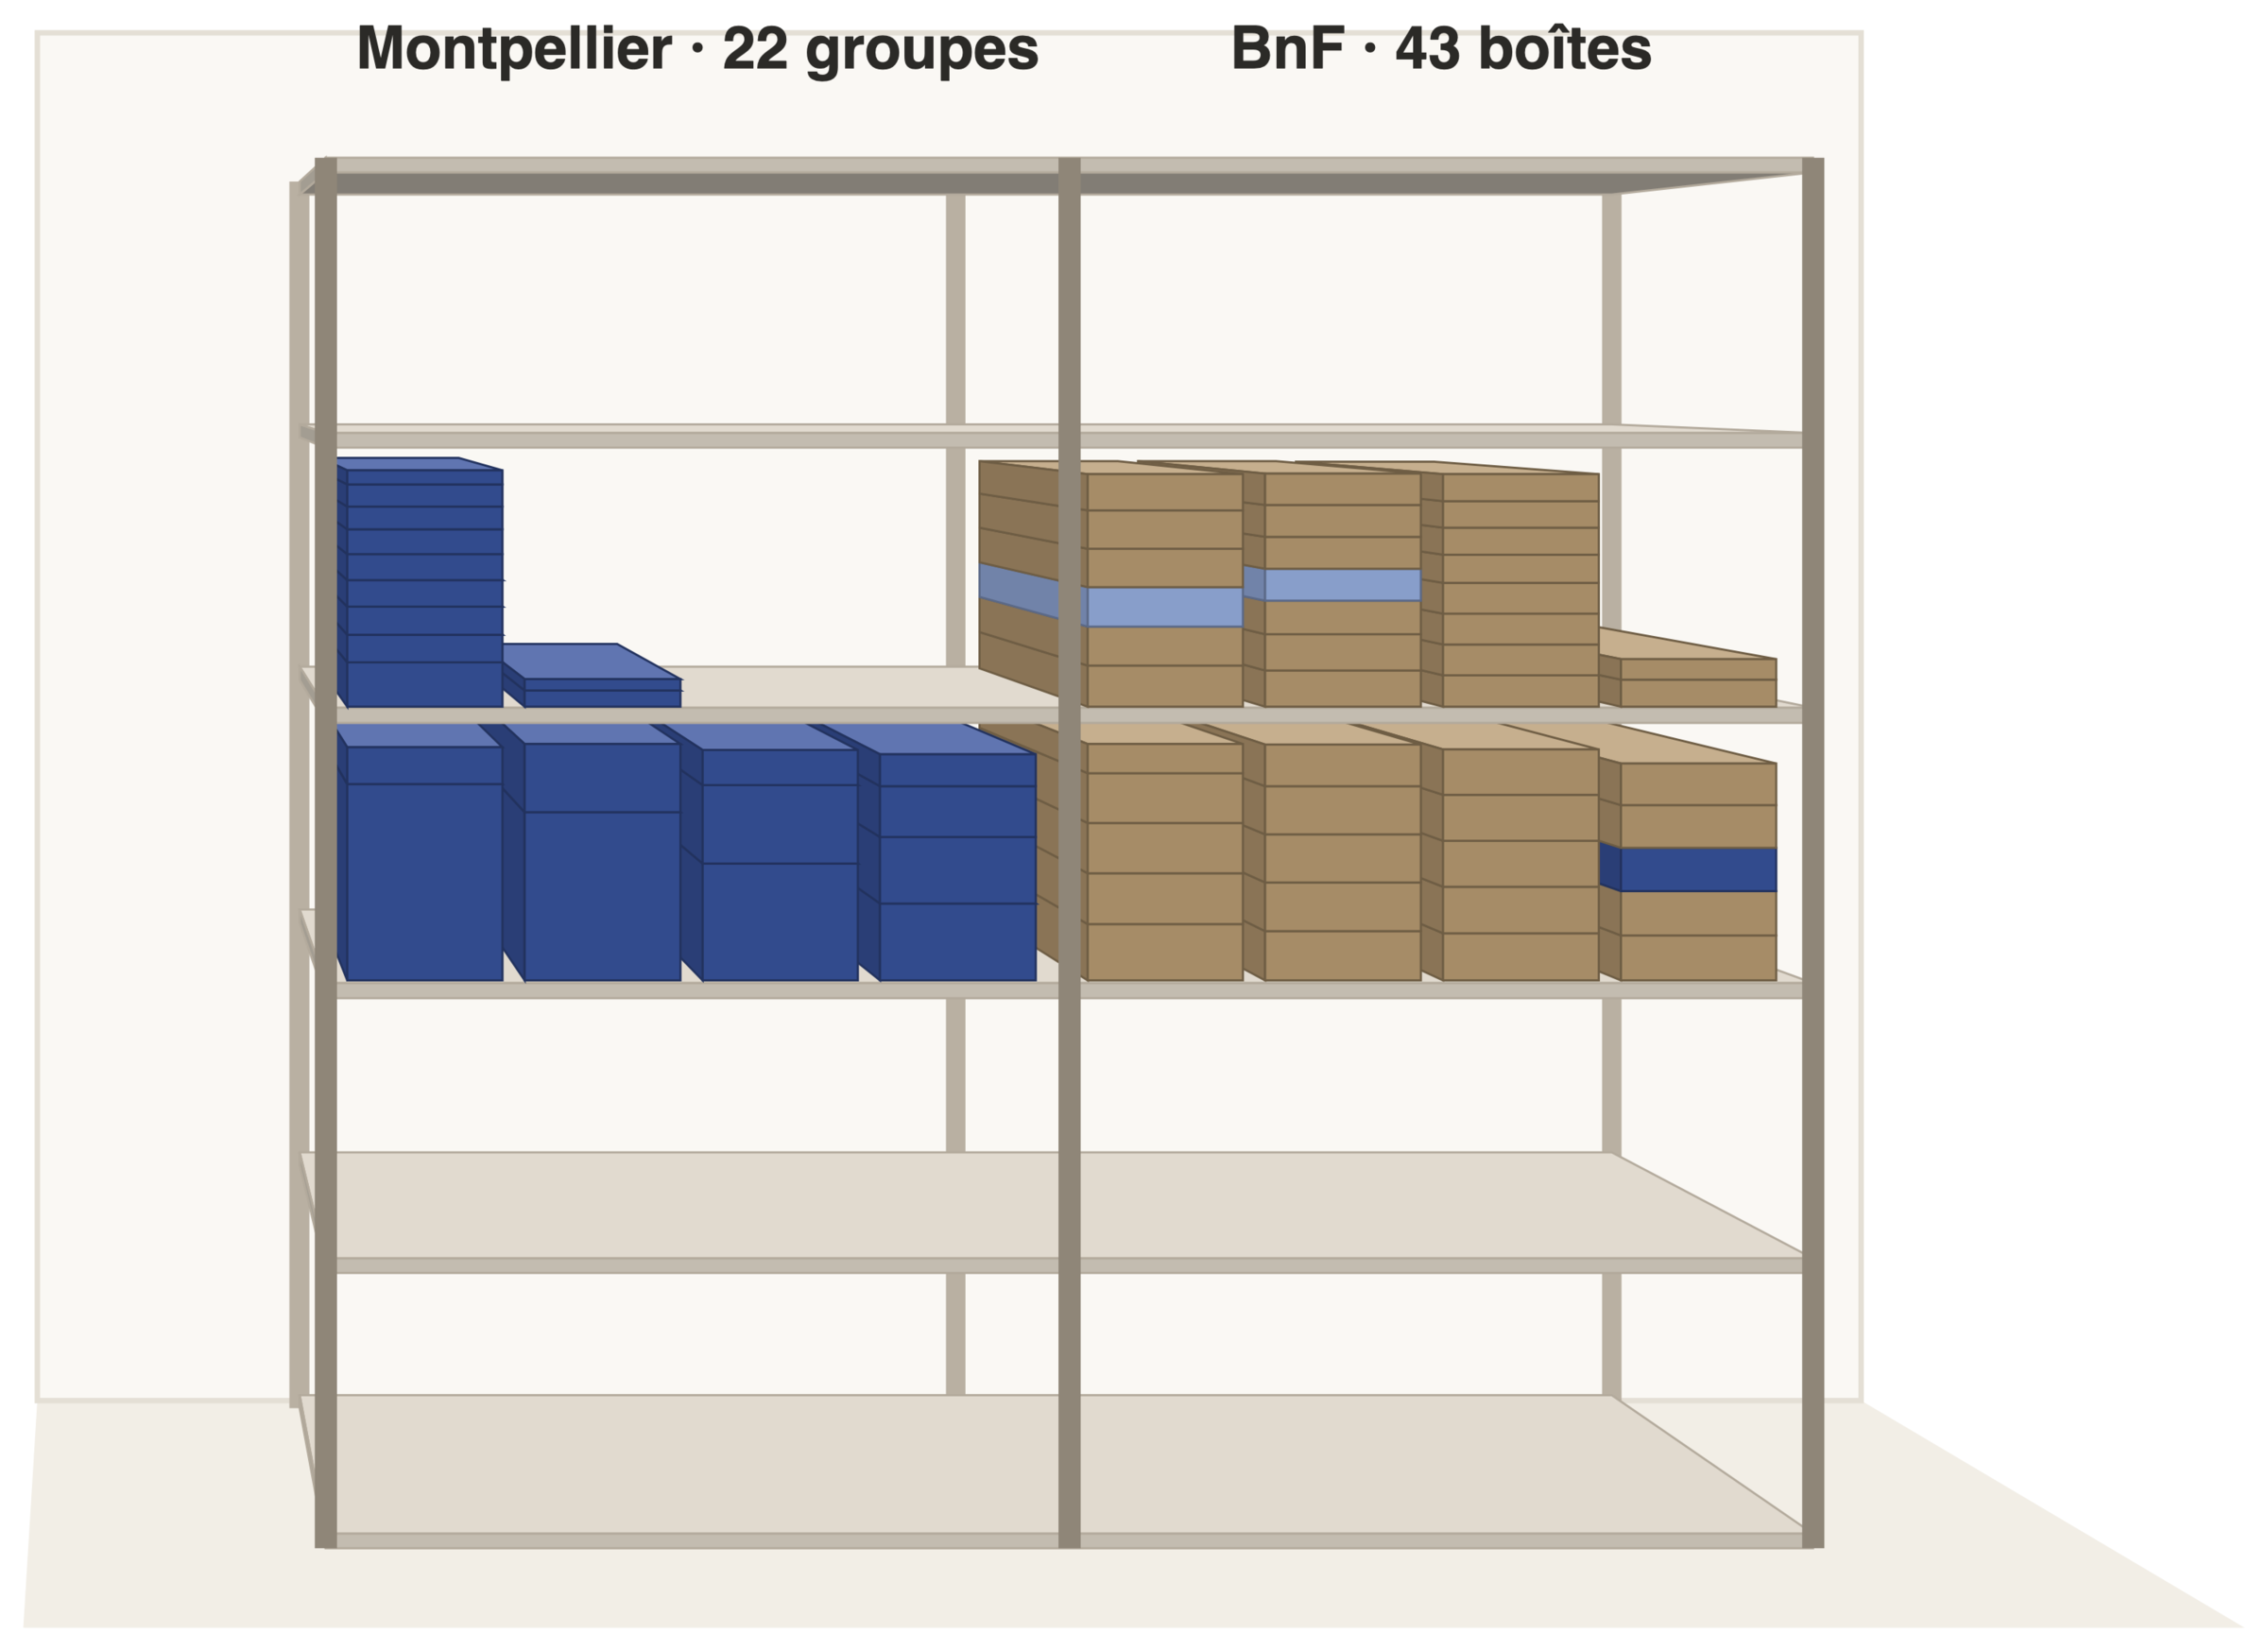
\includegraphics[width=\linewidth]{fig/etageres.png}\par\vspace{1.5mm}
\legende{\textbf{Tout tiendrait sur deux étagères.} Les deux fonds rangés dans une même réserve, à hauteur de bras. Chaque carton a le format d'une feuille A4 et la hauteur de sa pile de papier (un dixième de millimètre la feuille). À gauche, les 22 groupes de dossiers de Montpellier, tous mathématiques ; à droite, les 43 boîtes de la BnF, en bleu clair celles qui contiennent un peu de mathématiques, en bleu foncé la seule qui en soit entièrement faite. Montpellier compte des pages et la BnF des feuillets : une pile de Montpellier peut être jusqu'à deux fois trop haute. Le papier seul est représenté.}\par\vspace{5mm}
\begin{multicols}{3}
\inter{Une machine en première lecture}
Depuis août 2026, un modèle de langage sert de premier lecteur. Il transcrit les dossiers par lots de vingt pages, en marquant ce qu'il a lu avec certitude, ce qu'il a deviné et ce qui reste illisible. Puis il rédige pour chaque dossier une lecture « modernisée », qui reformule les mathématiques dans les notations d'aujourd'hui. À ce jour, 165 dossiers sont transcrits.

Une troisième étape cherche dans la littérature les énoncés qui pourraient être nouveaux, une quatrième les fait vérifier par un logiciel de preuve. Ce sont ces deux étapes qui donnent au projet son intérêt : non pas seulement lire Grothendieck, mais confronter ce qu'il a écrit à ce que l'on sait aujourd'hui, et à ce qu'une machine peut vérifier.
\end{multicols}
\vfill
\begin{encadre}{En chiffres}
\textbf{178} dossiers à Montpellier, \textbf{16\,074} pages\\[1.5pt]
\textbf{43} boîtes à la BnF, \textbf{22\,495} feuillets\\[1.5pt]
\textbf{21} dossiers seulement datés de sa main, sur 164\\[1.5pt]
\textbf{456} énoncés recensés, dont \textbf{83} retrouvés dans la littérature\\[1.5pt]
plus de \textbf{2\,000} théorèmes vérifiés par ordinateur\\[1.5pt]
\textbf{14} problèmes ouverts confiés aux mathématiciens
\end{encadre}
\foliog{2}}

% =================================================================== planche 2 (pages 3-4)
\planche{%
\rubrique{Une œuvre souterraine}
\grandtitre{Il n'a jamais arrêté d'écrire}
\centering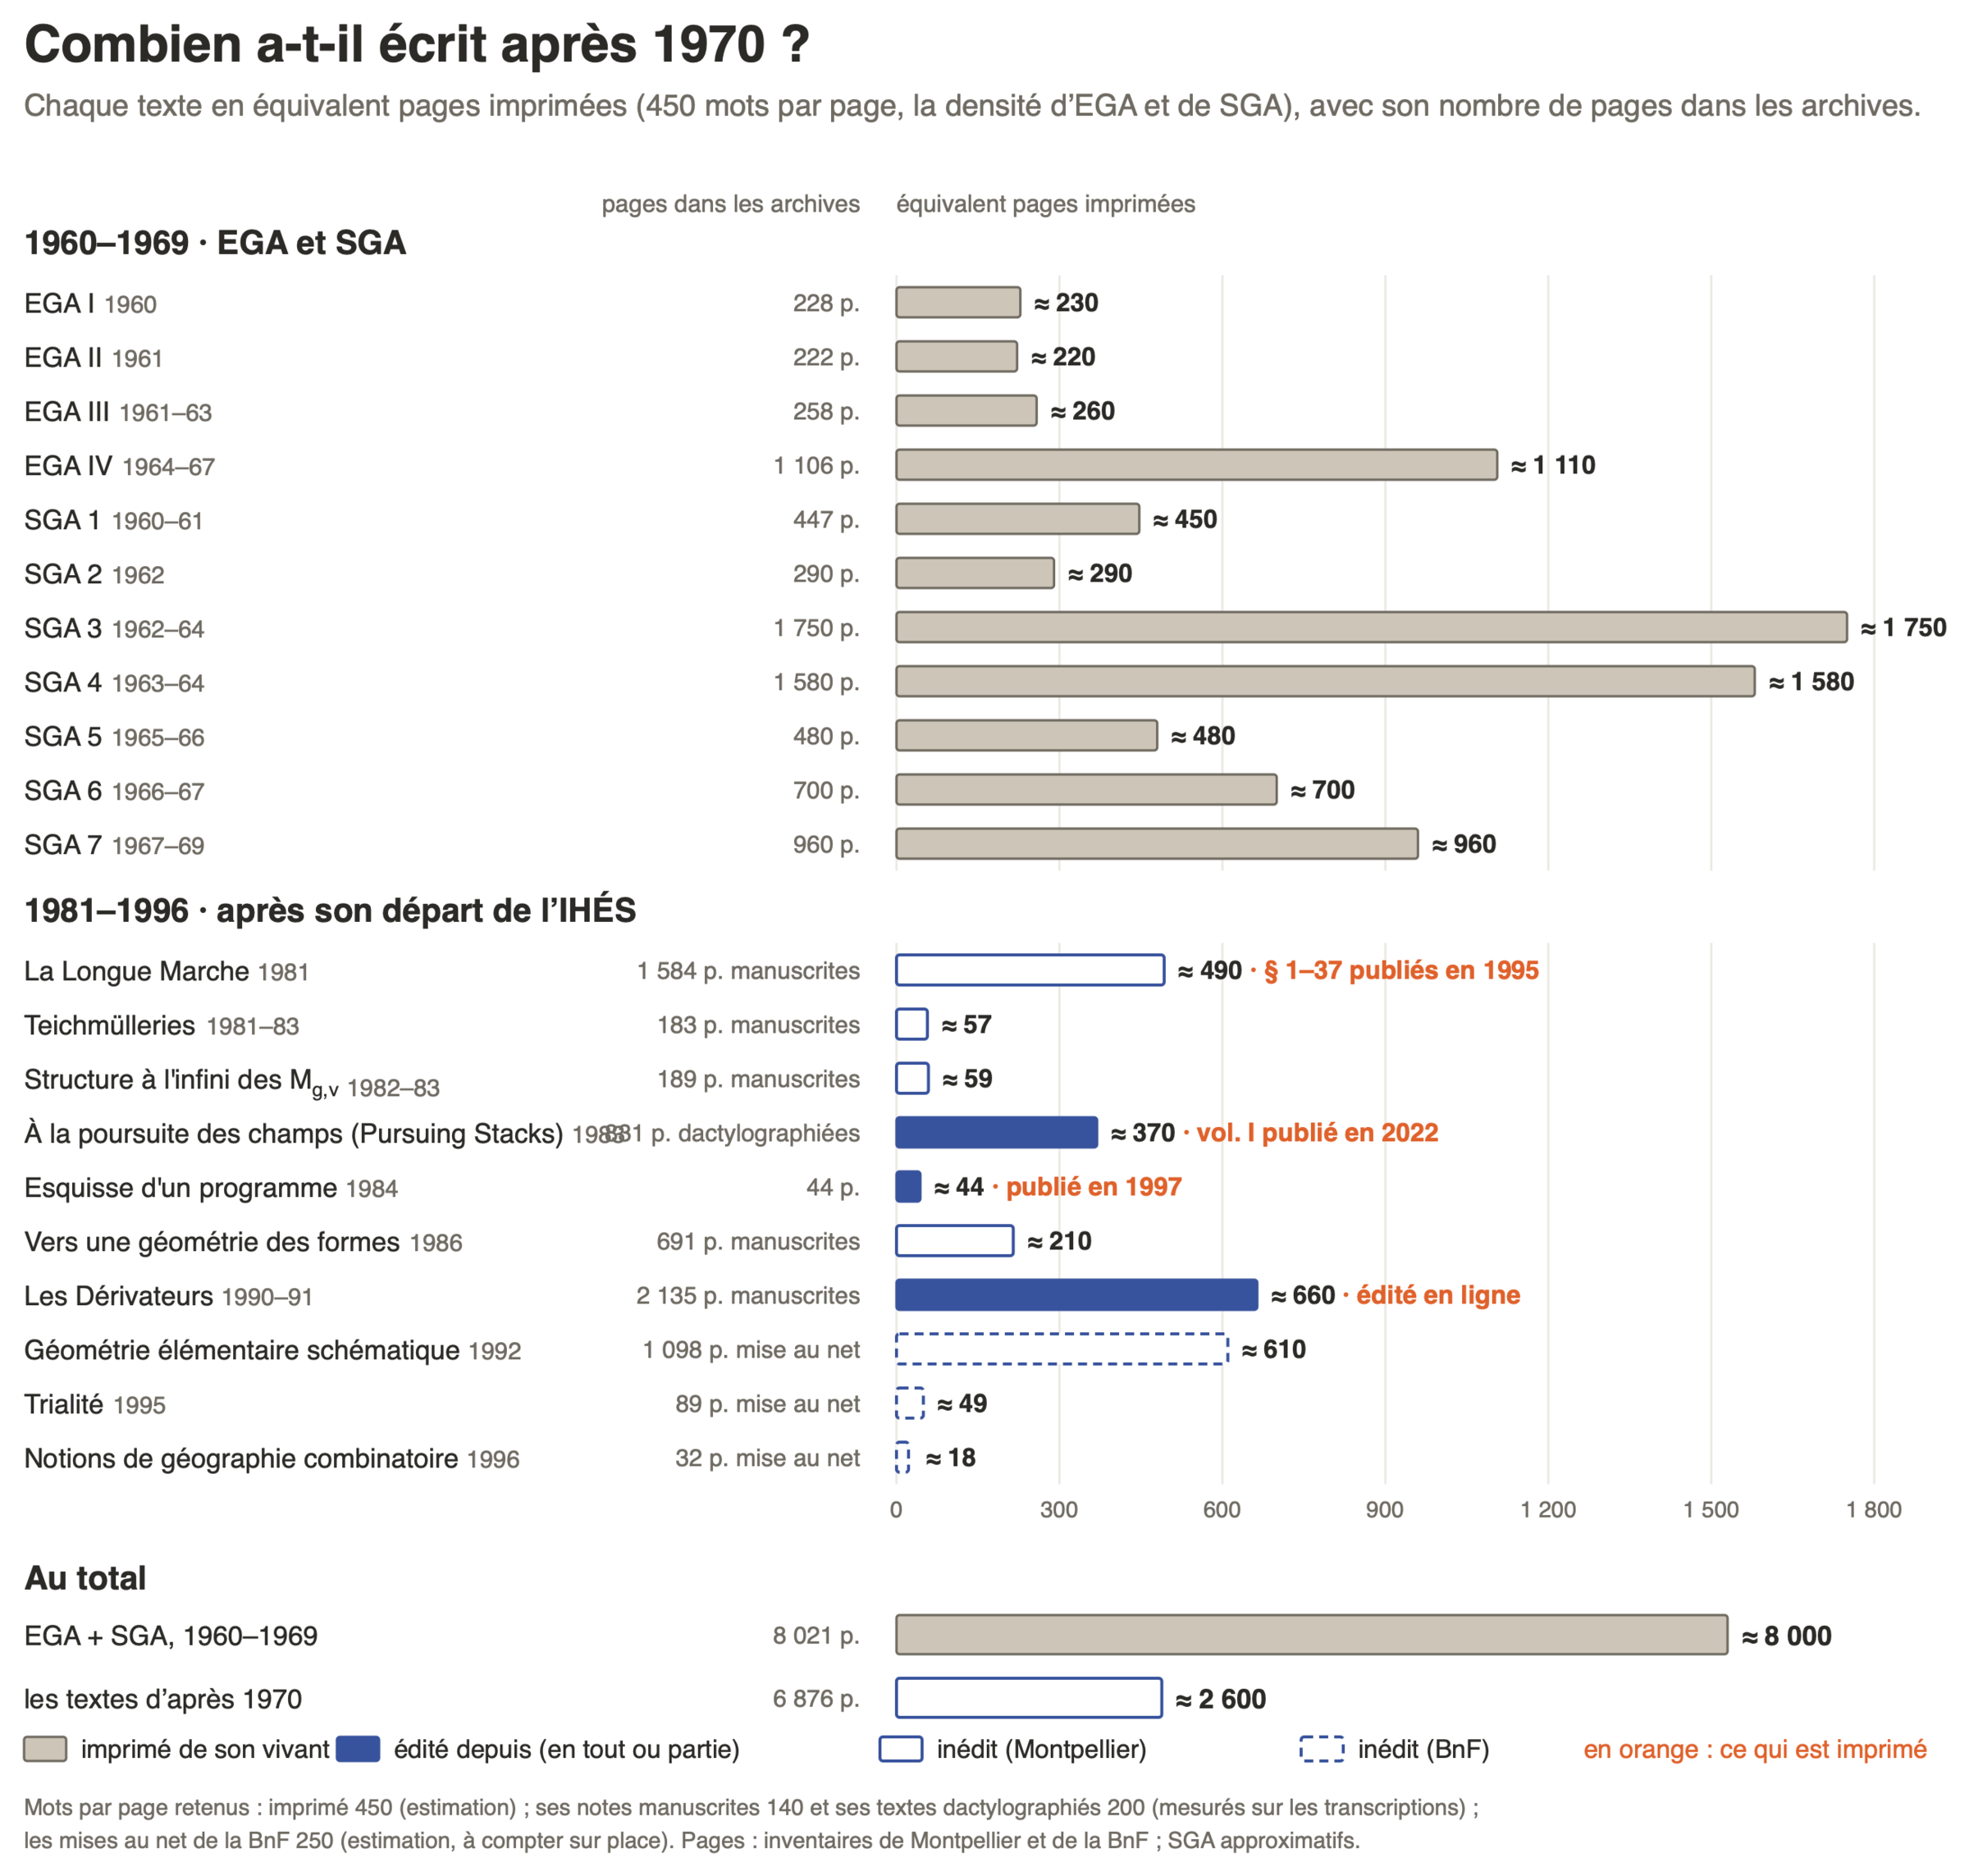
\includegraphics[width=0.9\linewidth]{fig/later-writing-fr.png}\par\raggedright\par\vspace{1.5mm}
\legende{\textbf{Combien a-t-il écrit après 1970 ?} Chaque texte est mesuré en équivalent pages imprimées, à 450 mots par page comme dans les EGA et SGA, pour comparer des manuscrits de densités différentes : environ 140 mots par page pour ses notes manuscrites, 200 pour ses textes tapés, ce qui est mesuré sur les transcriptions. Les longs textes écrits après son départ représentent environ un tiers des traités des années 1960. Les densités des mises au net de la BnF sont estimées.}\par\vspace{4mm}
\begin{multicols}{3}
Le premier constat est simple : il a continué. \emph{La Longue Marche à travers la théorie de Galois} (1981) fait près de 1\,600 pages manuscrites. \emph{À la poursuite des champs} (1983), tapé à la machine, en compte plus de 800. \emph{Les Dérivateurs} (1990--1991), plus de 2\,100.

Entre les deux, des textes restés inconnus du public, comme les \emph{Teichmülleries} ou \emph{Vers une géométrie des formes}, écrit en juin et juillet 1986, où il cherche une géométrie sans points, faite de morceaux et de leurs contacts.

Les cartons de la BnF prolongent l'histoire jusqu'en 1999, mais changent de nature. L'essentiel est une méditation philosophique et spirituelle, \emph{La Clef des Songes} puis \emph{Le Problème du Mal}, sur des milliers de feuillets. Les mathématiques n'y reviennent que par épisodes : une \emph{Géométrie élémentaire schématique} de 1992, d'une écriture soignée, une \emph{Trialité} en 1995, des \emph{Notions de « géographie combinatoire »} en 1996, et des « bitrialités » notées encore en février 1998.
\end{multicols}
\foliog{3}}{%
\vspace*{12mm}
\begin{multicols}{3}
\inter{Une manière de travailler}
Les pages datées montrent comment il travaillait. Il note la date de ses séances, garde ses faux départs et les numérote, mène plusieurs sujets de front. Il écrit pour lui, vite, en abrégeant, et revient sur ce qu'il a écrit la veille.

Pendant l'hiver 1983--1984, par exemple, il alterne d'une semaine à l'autre entre les groupes de Teichmüller, la structure des dérivateurs, des courbes elliptiques réelles, des questions de géométrie combinatoire et la chirurgie des surfaces, tout en corrigeant le tapuscrit d'\emph{À la poursuite des champs}. C'est le même hiver qu'il date l'\emph{Esquisse d'un programme}, l'un de ses textes les plus célèbres.

Et il reconnaît ses erreurs sur la page, sans détour.

\exergue{Faux\,! idiot\,!}
{\sans\fontsize{8}{10}\selectfont\color{gris}En marge d'une page du 6 juin 1986.}\par\medskip

Le 3 janvier 1984, après onze jours sur un problème de courbes, il écrit simplement : «\,je m'étais mélangé les pinceaux \emph{deux} fois, il me semble\,». Ailleurs : «\,C'est ultra faux\,», suivi d'un contre-exemple à trois éléments.

Ces traces de travail, qui n'apparaissent dans aucun livre, sont peut-être ce que les archives ont de plus précieux. Elles montrent un mathématicien qui se trompe, revient en arrière et recommence, loin de l'image du génie infaillible.
\end{multicols}
\vspace{4mm}
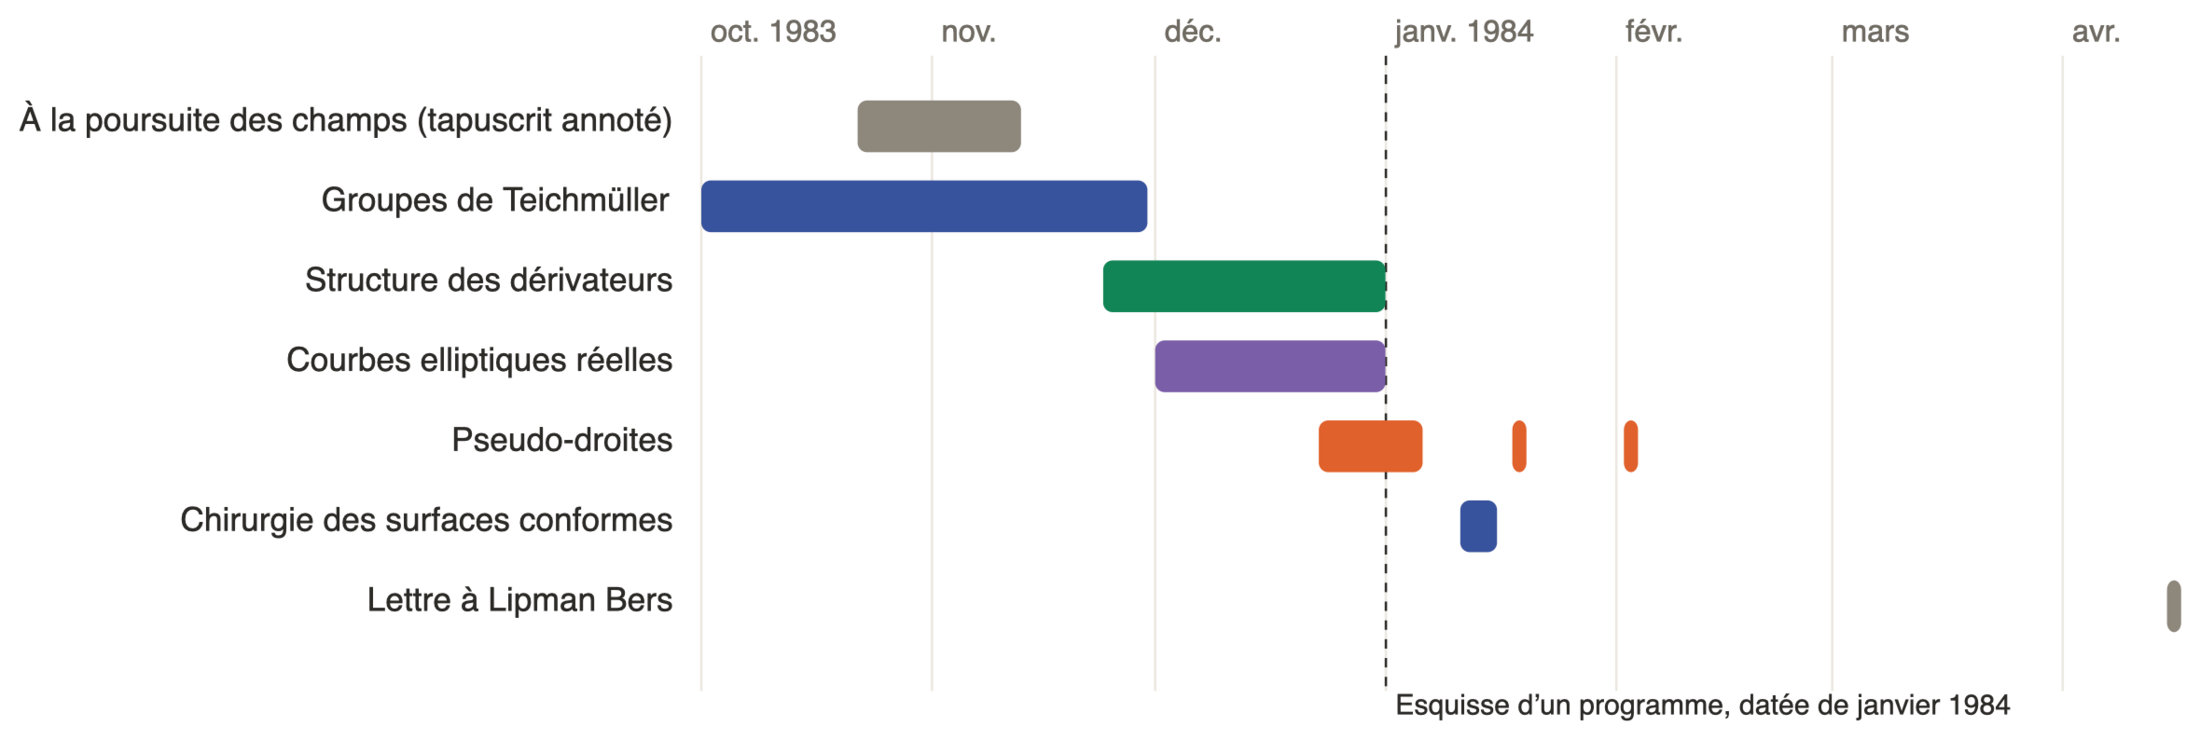
\includegraphics[width=\linewidth]{fig/hiver.png}\par\vspace{1.5mm}
\legende{\textbf{L'hiver 1983--1984, d'après les feuillets qu'il a datés.} Sept sujets en quelques mois, dont trois reprises du même problème de pseudo-droites. La ligne pointillée marque janvier 1984, date de l'\emph{Esquisse d'un programme}. Les archives ne disent pas dans quel ordre il pensait à tout cela, seulement quand il l'a écrit.}
\folio{4}}

% =================================================================== planche 3 (pages 5-6)
\planche{%
\rubrique{Ce que la littérature savait déjà}
\grandtitre{Seize mille pages au tamis}
{\centering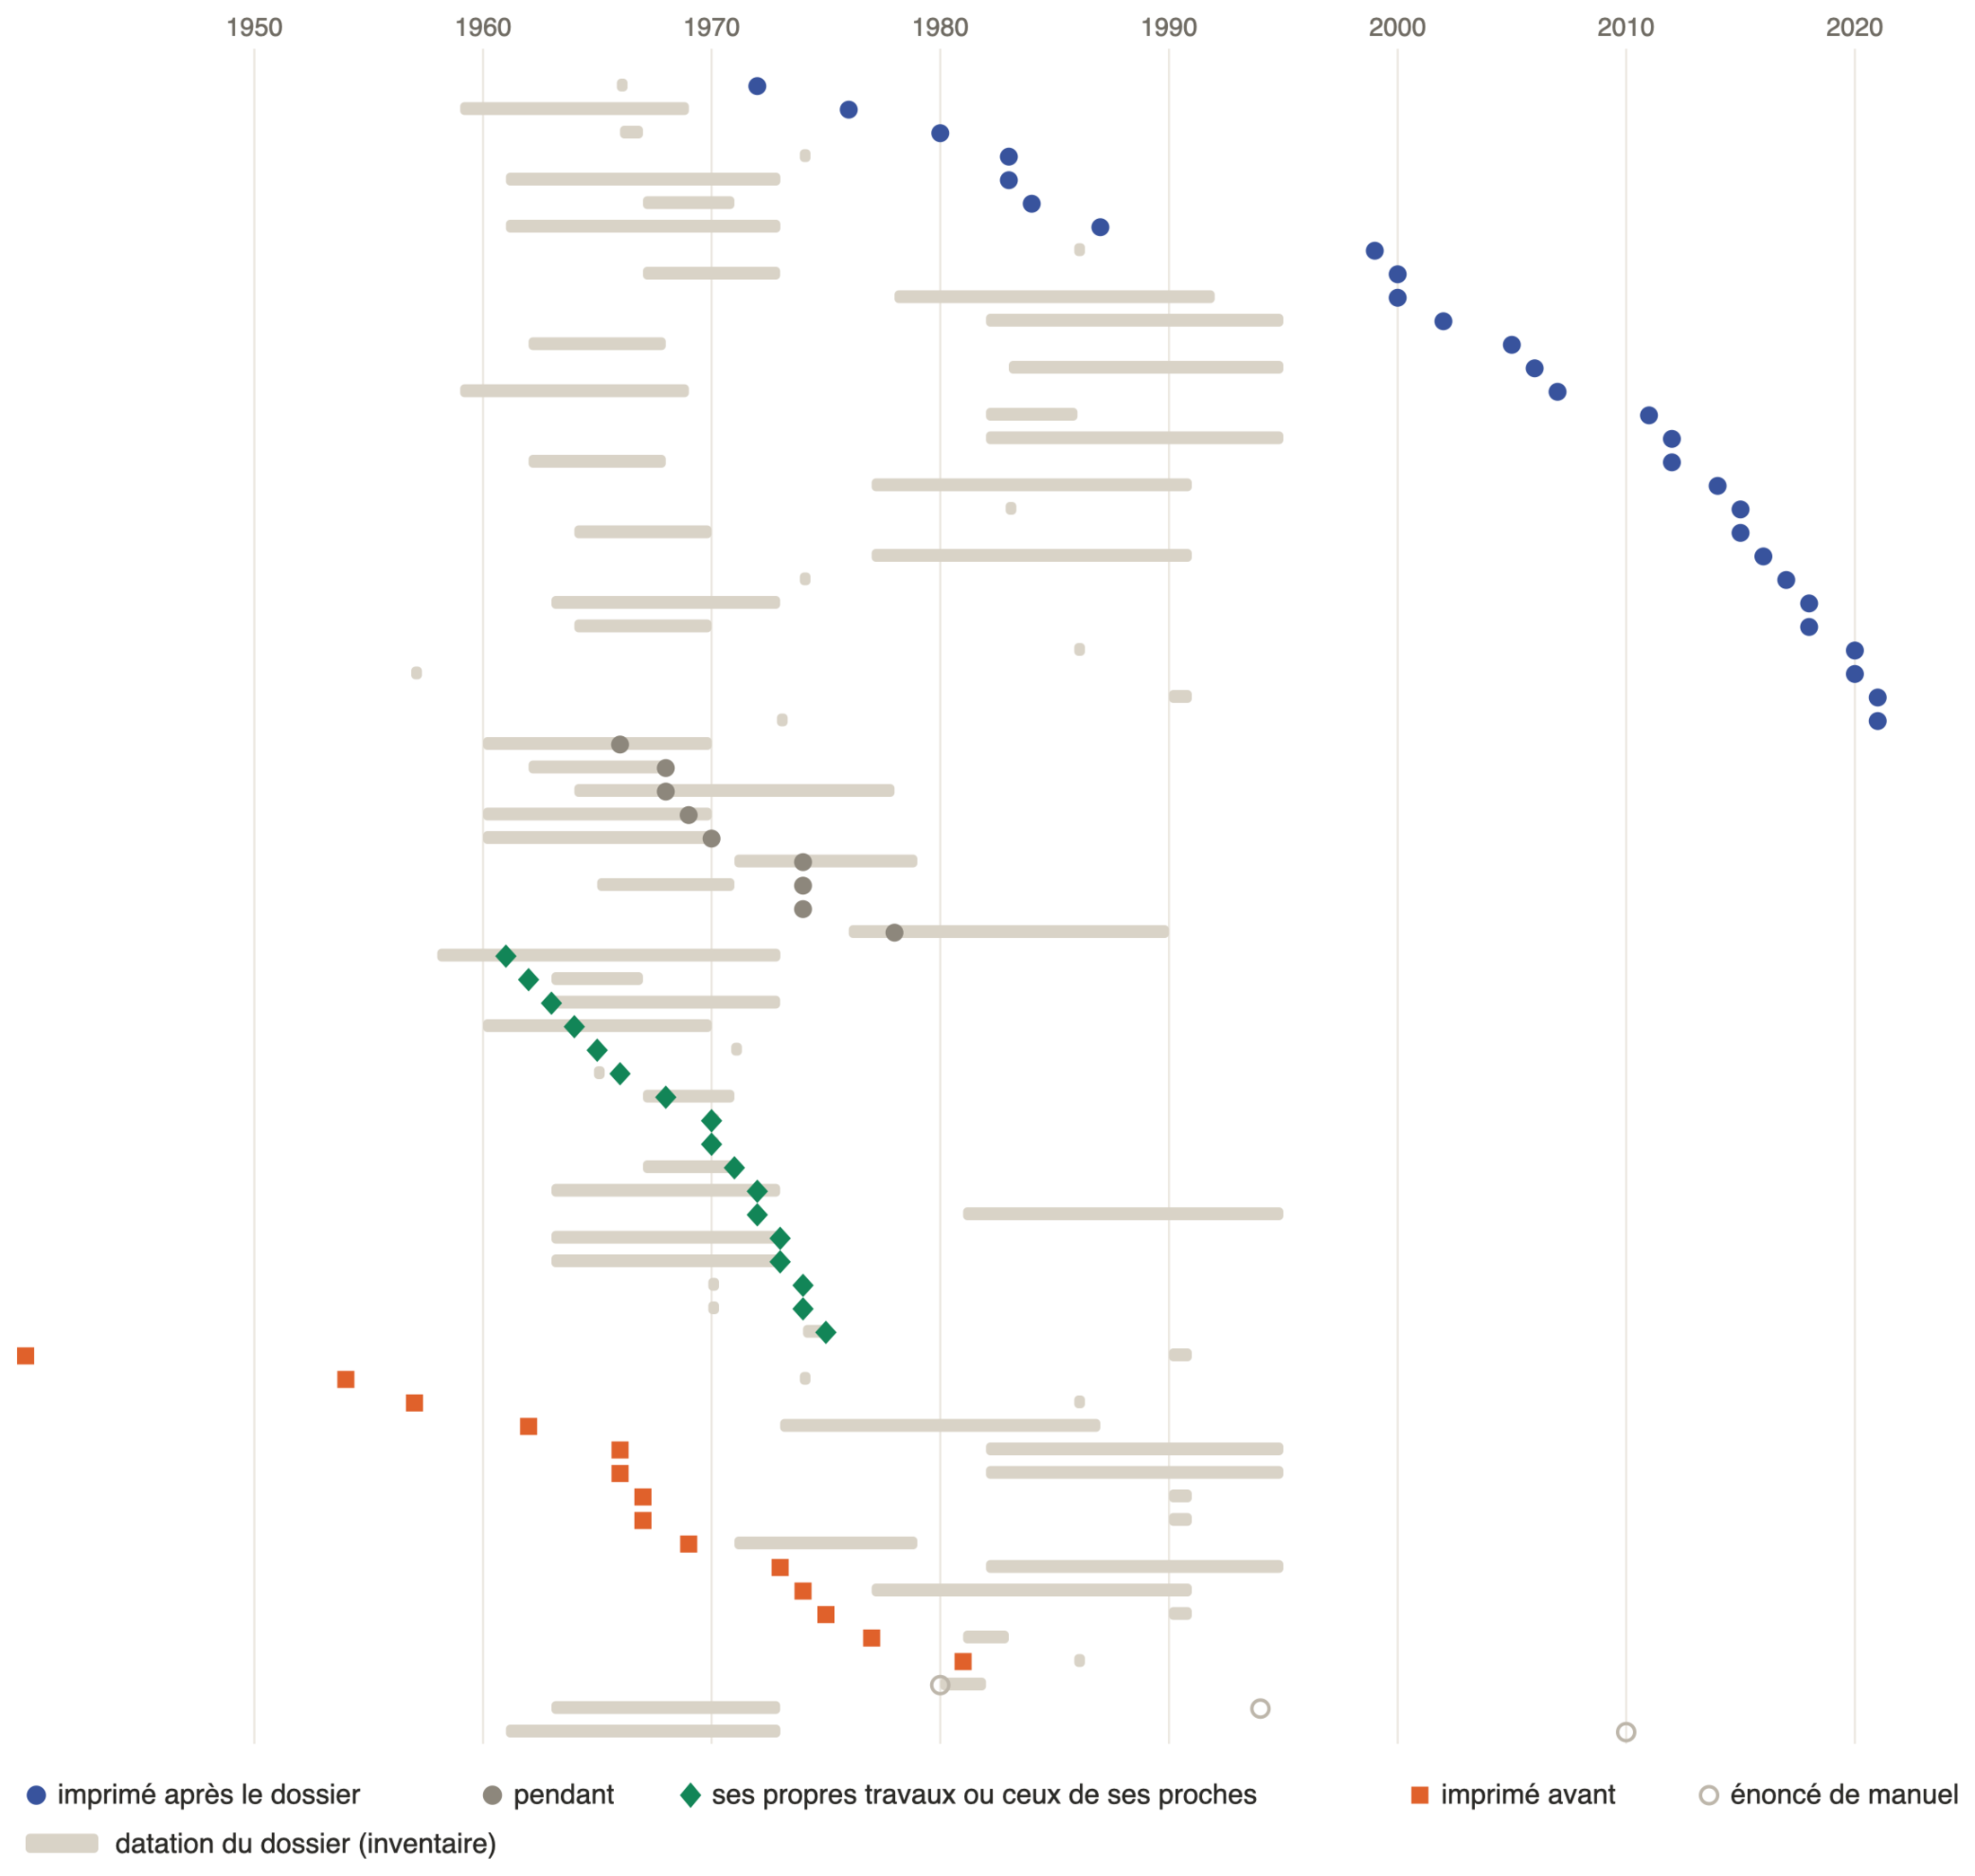
\includegraphics[width=0.8\linewidth]{fig/retrouves.png}\par}\par\vspace{1.5mm}
\legende{\textbf{71 énoncés des brouillons retrouvés dans les livres.} Chaque ligne oppose la datation du dossier (barre grise) à l'année de la publication qui contient le même résultat (point). En bleu, ce qui a été imprimé après le dossier, souvent des décennies plus tard ; en orange, avant : Grothendieck refait alors dans sa notation un résultat déjà connu ; en vert, ses propres travaux ou ceux de ses proches. Les datations sont celles de l'inventaire, souvent déduites : aucune priorité n'est revendiquée. Les sources antérieures à 1940 sont ramenées au bord gauche.}
\vfill
\begin{encadre}{Une démonstration sans mots}
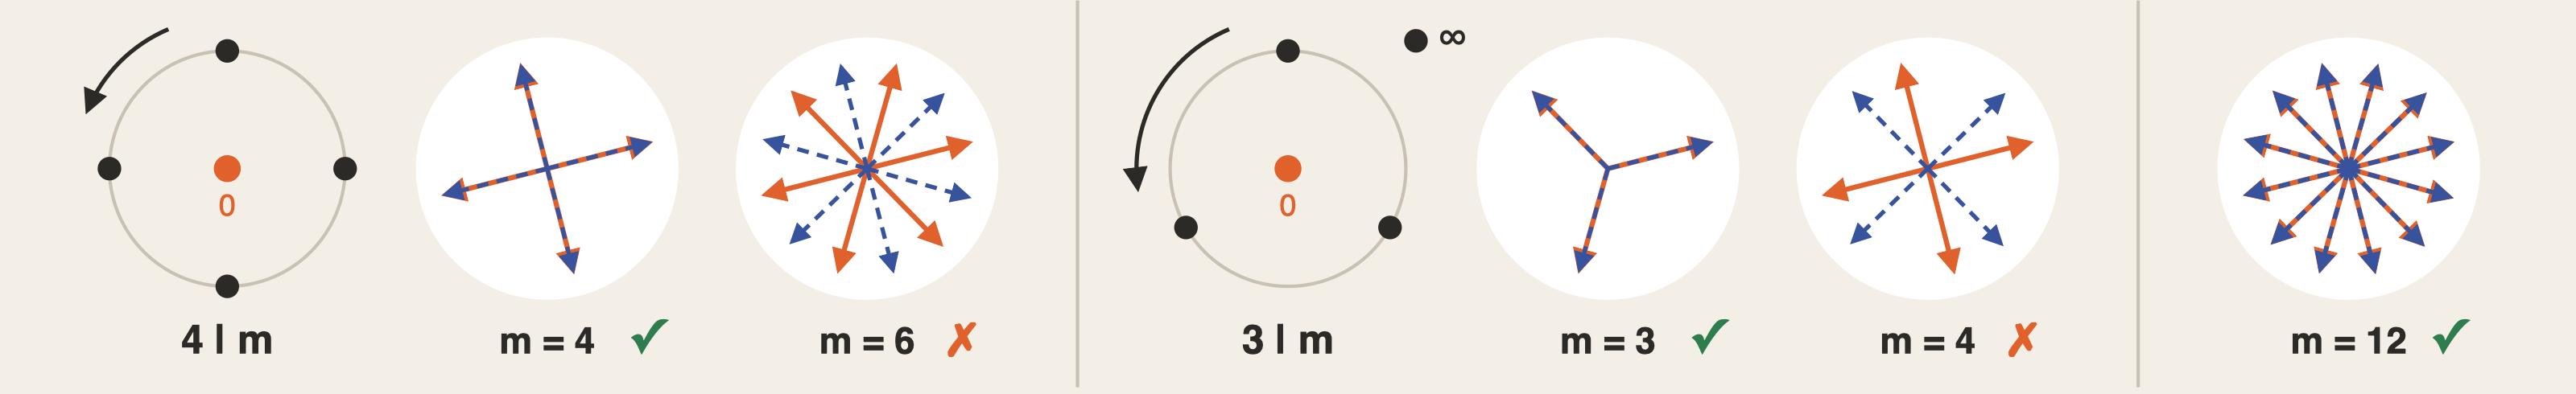
\includegraphics[width=\linewidth]{fig/sans-mots-146-bandeau.png}\par\vspace{2mm}
Vers 1978, dans les \emph{Groupoïdes de Teichmüller}, Grothendieck dresse le tableau des plus petites puissances qui rendent trivial un certain fibré attaché à $n$ points sur la sphère ; pour cinq points, il note « 12 ? », et l'édition a démontré que c'est juste. Mettez l'un des points au centre (en orange) et faites tourner la figure : le vecteur tangent au centre tourne avec elle, et sa puissance $m$-ième, dessinée comme une étoile à $m$ branches, doit retomber sur elle-même (en bleu, l'étoile tournée). Le quart de tour impose que 4 divise $m$, le tiers de tour, avec un point à l'infini, que 3 divise $m$ : il faut $m = 12$. Pour $n$ points on trouve $(n-1)(n-2)$, ce que Lean vérifie dans un modèle algébrique de la situation ; pour six points, Grothendieck proposait 60 au lieu de 20.
\end{encadre}
\foliog{5}}{%
\vspace*{12mm}
\begin{multicols}{3}
Une troisième étape cherche dans la littérature les énoncés qui pourraient être nouveaux. Le registre en compte aujourd'hui 456. Pour 83 d'entre eux, la recherche a montré qu'ils étaient déjà imprimés.

Sur les 71 premiers rapprochements, 28 publications sont postérieures aux dates de l'inventaire, souvent de plusieurs décennies ; 14 sont antérieures, et Grothendieck redémontre le résultat dans sa propre notation sans le citer ; 17 viennent de ses propres publications ou de celles de ses élèves. Aucun de ces rapprochements n'est une revendication de priorité : les dates des dossiers sont trop incertaines pour cela.

\inter{Lean, le relecteur intraitable}
Reste à savoir si ces énoncés sont justes. Pour cela, l'édition utilise Lean, un logiciel qui vérifie une démonstration pas à pas, sans rien laisser passer, en s'appuyant sur une immense bibliothèque de résultats déjà vérifiés, Mathlib. Plus de deux mille théorèmes tirés des dossiers y ont été démontrés.

Lean a aussi servi de détecteur d'erreurs. Il a trouvé des lectures fautives de la machine, des glissements dans les pages elles-mêmes, et quelques affirmations de Grothendieck qui sont fausses telles qu'il les a écrites. Sur ses pages de 1981 consacrées aux pseudo-droites, par exemple, un « théorème » se révèle faux : six droites bien choisies le contredisent, et Lean le vérifie.



\inter{Quatorze énigmes}
Lean ne peut vérifier qu'un énoncé dont les objets existent dans sa bibliothèque. Or Grothendieck travaillait justement là où elle s'arrête : cohomologie étale, champs, topos, motifs. Près d'une centaine d'énoncés restent ainsi hors de portée. Quatorze, parmi les plus précis, ont été rassemblés dans un document à l'intention des mathématiciens, avec pour chacun la page du manuscrit, ce que l'on sait, et ce qui permettrait de trancher.

\begin{encadre}{Comment lire une page de Grothendieck}
Une page typique mêle phrases, formules et schémas. La transcription garde trace de tout ce qui est incertain : un mot deviné, un mot illisible, un passage biffé, un ajout dans la marge. Rien n'est corrigé en silence. La lecture modernisée, elle, peut réécrire, mais chaque écart avec la page est signalé en note. Quand la lecture et la page divergent, c'est la page qui fait foi.
\end{encadre}

\inter{Les droits, une question ouverte}
Les fac-similés de Montpellier sont publics. Les transcriptions, elles, ne le sont pas : les droits appartiennent aux héritiers de Grothendieck, et aucune transcription ne peut être mise en ligne sans leur autorisation. Les lectures restent donc, pour l'instant, un outil de travail : on peut les citer brièvement, pas les publier.
\end{multicols}
\vfill
\begin{encadre}{Le « théorème » faux de 1981}
\begin{minipage}[t]{0.42\linewidth}\vspace{0pt}
\begin{tikzpicture}[scale=0.95]
\disque
\coordinate (A) at (-0.9,-0.6); \coordinate (B) at (1.0,-0.55); \coordinate (C) at (0.05,0.95);
\ligne{A}{B} \ligne{B}{C} \ligne{C}{A}
\ligne[orange]{A}{$(A)+(1,0.75)$} \ligne[orange]{B}{$(B)+(-0.35,1)$} \ligne[orange]{C}{$(C)+(0.95,-0.2)$}
\foreach \c/\d in {A/below left,B/below right,C/above left} \fill (\c) circle (2pt) node[\d,font=\sffamily\scriptsize]{$\c$};
\end{tikzpicture}
\end{minipage}\hfill
\begin{minipage}[t]{0.55\linewidth}\vspace{0pt}
Sur la page 24 de ses notes de 1981, Grothendieck énonce un théorème sur les arrangements de pseudo-droites. Six droites suffisent à le contredire : les trois côtés d'un triangle $ABC$ (en bleu) et trois droites passant chacune par un sommet (en orange), sans point commun. Chaque droite y porte au moins trois croisements, mais l'arrangement n'a pas la forme annoncée. Lean vérifie le contre-exemple en coordonnées entières. L'énoncé qu'il en tirait, lui, reste vrai : c'est le théorème expliqué plus loin.
\end{minipage}
\end{encadre}
\folio{6}}

% =================================================================== planche 4 (pages 7-8)
\planche{%
\rubrique{Le théorème expliqué}
\grandtitre{Les droites qui n'en sont pas}
\chapo{En 1981, Grothendieck s'intéresse à des courbes qui se comportent comme des droites. Il énonce un résultat sans le démontrer. Quarante-cinq ans plus tard, la preuve tient en quelques lignes.}
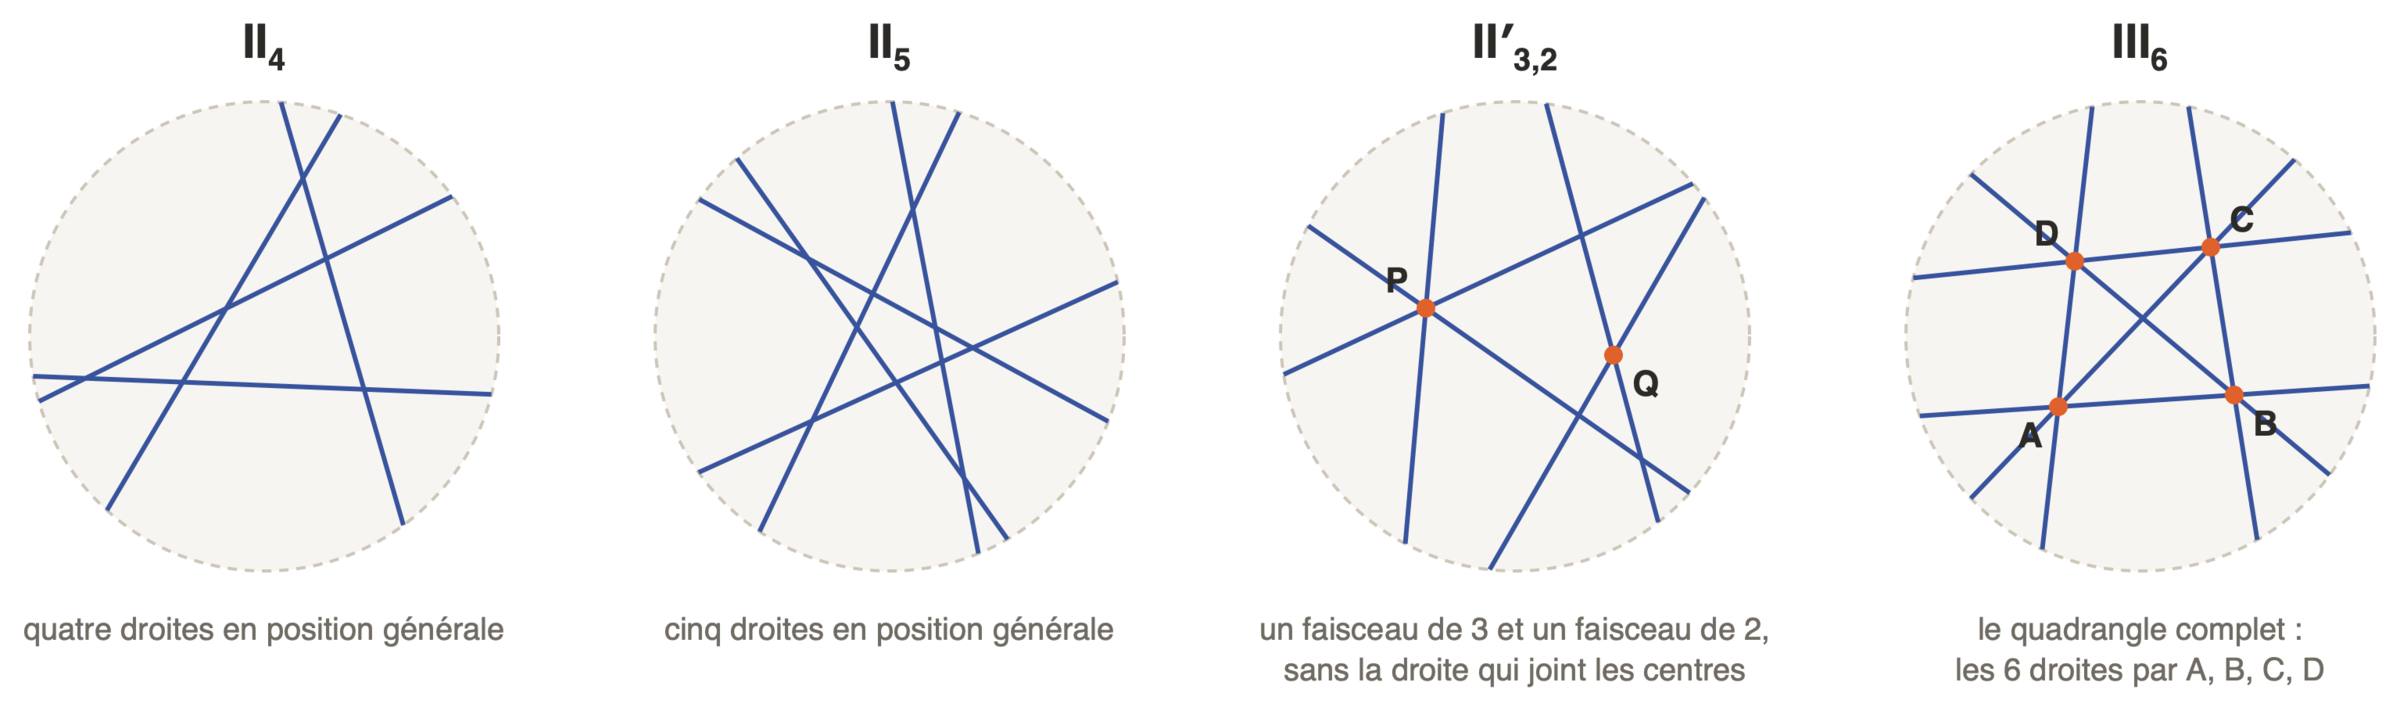
\includegraphics[width=\linewidth]{fig/bigon-configurations-fr.png}\par\vspace{1mm}
\legende{Les quatre dessins de Grothendieck. Dans chacun, toute courbe porte au moins trois croisements. Les points orange marquent les endroits où trois courbes se croisent.}\par\vspace{3mm}
\begin{multicols}{2}
Tracez sur une feuille des courbes qui ne sont pas forcément droites, mais qui se croisent deux à deux exactement une fois, comme le feraient des droites. Pour que deux courbes « parallèles » se croisent aussi, on travaille dans le plan projectif, un plan où l'horizon est recollé à lui-même. Ces courbes s'appellent des pseudo-droites.

Grothendieck s'intéresse aux dessins où chaque courbe porte au moins trois points de croisement. Il affirme qu'un tel dessin est soit fait de quatre courbes en position générale, soit contient l'un des trois motifs ci-dessus : cinq courbes en position générale, un faisceau de trois et un faisceau de deux, ou le quadrangle complet, les six droites qui passent par quatre points. Mais la démonstration qu'il en donne s'appuie sur un autre énoncé de la même page, qui est faux.

\textbf{L'outil : un vieux théorème.} Sylvester demande en 1893 si, dans tout ensemble de droites qui ne passent pas toutes par un même point, il existe un point où ne se croisent que deux d'entre elles. La réponse est oui ; elle est démontrée au XX\textsuperscript{e} siècle, et reste vraie pour les pseudo-droites.

\textbf{La preuve en trois temps.} On part de ce point où deux courbes seulement se croisent, et on en déduit quatre courbes dont trois ne passent jamais par un même point. Une cinquième courbe passe alors par zéro, un ou deux de leurs six croisements :
\end{multicols}
\vspace{2mm}
\noindent\begin{tikzpicture}[scale=0.92]
\foreach \k/\tit/\res in {0/{aucun croisement}/{cinq courbes en position générale},1/{un croisement}/{un faisceau de 3 et un de 2},2/{deux croisements}/{une « diagonale »}} {
\begin{scope}[xshift=\k*6.15cm]
\begin{scope}
\disque
\coordinate (P1) at (-0.75,-0.6); \coordinate (P2) at (0.9,-0.45); \coordinate (P3) at (0.7,0.75); \coordinate (P4) at (-0.6,0.6);
\ligne{P1}{P2} \ligne{P2}{P3} \ligne{P3}{P4} \ligne{P4}{P1}
\ifnum\k=0 \ligne[orange]{-2,0.1}{2,-0.3} \fi
\ifnum\k=1 \ligne[orange]{P1}{$(P1)+(1,0.35)$} \fill[orange] (P1) circle (2.4pt); \fi
\ifnum\k=2 \ligne[orange]{P1}{P3} \fill[orange] (P1) circle (2.4pt); \fill[orange] (P3) circle (2.4pt); \fi
\end{scope}
\node[font=\sffamily\small\bfseries] at (0,-1.95) {\tit};
\node[font=\sffamily\scriptsize,text=gris] at (0,-2.35) {\res};
\end{scope}}
\end{tikzpicture}\par\vspace{2mm}
\begin{multicols}{2}
Dans les deux premiers cas, on tient l'un des motifs. Dans le troisième, la cinquième courbe est une diagonale du quadrilatère formé par les quatre premières. Une diagonale seule ne porterait que deux croisements, ce qui est interdit ; deux diagonales forment le quadrangle complet. Le théorème est démontré.

\noindent{\sans\fontsize{8.6}{11}\selectfont\color{gris}Cette preuve a été écrite par l'édition et vérifiée par ordinateur dans un modèle combinatoire des dessins. Aucun spécialiste ne l'a encore relue.}
\end{multicols}
\foliog{7}}{%
\vspace*{12mm}
\begin{encadre}{Une énigme encore ouverte}
Sur les mêmes pages, Grothendieck pose une question plus difficile : si l'on oublie le dessin et qu'on ne garde que la liste des croisements et des segments, avec le nom de la courbe qui porte chaque segment, peut-on redessiner l'arrangement, et chaque symétrie de cette liste vient-elle d'une symétrie du dessin ? La réponse est oui quand aucun point ne réunit plus de deux courbes : c'est démontré et vérifié par ordinateur. Pour les autres dessins, c'est encore ouvert. La question est posée sur le forum MathOverflow.
\end{encadre}\par\vspace{3mm}
\begin{multicols}{3}
\inter{Ce que la machine ne sait pas faire}
La machine lit vite, mais elle lit mal ce qu'elle ne connaît pas. Une note de 1970 affirme qu'un certain groupe d'extensions s'annule. Le modèle a cherché plusieurs fois dans la littérature, a conclu que la question était ouverte, et a manqué un article de Lawrence Breen paru en 1975 qui la règle presque entièrement. Un spécialiste l'aurait sans doute cité de mémoire.

Une vérification systématique des références d'un document de travail a trouvé dix attributions fausses sur une trentaine : des théorèmes cités au mauvais numéro, des résultats prêtés à un livre qui ne les contient pas. La machine est très sûre d'elle, même quand elle se trompe. C'est pourquoi chaque lecture douteuse est signalée, chaque argument de l'édition marqué comme tel, et chaque énoncé confronté à la page.

\inter{Et maintenant}
Le projet continue : transcrire les derniers dossiers, vérifier sur les fac-similés les lectures douteuses, et retourner à la BnF pour mesurer ce que contiennent les boîtes mathématiques, pochette par pochette.

Surtout, il faut que des mathématiciens s'emparent de ces pages. La machine peut lire, classer, vérifier ; elle ne sait pas encore dire ce qui compte. Grothendieck écrivait pour lui-même ; quarante ans plus tard, ses brouillons attendent toujours leurs lecteurs.
\end{multicols}
\vfill
{\titre\color{orange}\fontsize{26}{31}\selectfont «\,Je n'ai donc pas vérifié que la proposition énoncée soit correcte.\,»\par}\vspace{1mm}
{\sans\fontsize{9}{11}\selectfont\color{gris}Grothendieck, notes sur les pseudo-droites, 1981 (Montpellier, cote 80, p.~48).}\par
\vfill
\begin{encadre}{Pour aller plus loin}
Les fac-similés du fonds de Montpellier sont en libre accès sur le site de l'université : \emph{grothendieck.umontpellier.fr}. Les notices du fonds de la BnF (NAF 29093) sont consultables sur \emph{archivesetmanuscrits.bnf.fr}. La biographie de référence en ligne est celle de MacTutor (université de St Andrews).
\end{encadre}
\folio{8}}

\end{document}
